[10~v\textsuperscript{o}]
progressioni, Elateres\protect\index{Sachverzeichnis}{elater} per\textso{ harmonicam }reguntur;\textso{ Geometricam }ego primus reperi
\edtext{in\textso{ Detrimento.}}{\lemma{in}\Bfootnote{\textit{(1)}\ attritu \textit{(2)}\ \textso{Detrimento.} \textit{L}}}
\pend
\count\Bfootins=1000
\count\Afootins=1200
\pstart 
Nam \edtext{gravia\protect\index{Sachverzeichnis}{grave} labentia}{\lemma{gravia}\Bfootnote{\textit{(1)}\ aequali \textit{(2)}\ uniformiter crescentia \textit{(3)}\ labentia, \textit{L}}},
vires\protect\index{Sachverzeichnis}{vis} habent arithmetica progressione crescentes:
si Elaterem tendes, resistentiam\protect\index{Sachverzeichnis}{resistentia} crescere senties harmonica progressione.
Si naviculam in liquido \edtext{aut pilam}{\lemma{aut}\Bfootnote{\textit{(1)}\ navem \textit{(2)}\ pilam \textit{L}}}
in plano \edtext{horizontali}{\lemma{}\Bfootnote{horizontali \textit{erg.} \textit{L}}}
\edtext{propellas, Geometricam proportionem detrimenti virium deprehendes}{\lemma{propellas,}\Bfootnote{\textit{(1)}\ senties \textit{(2)}\ Geometricam [...] deprehendes, \textit{L}}},
irrefragabili demonstratione.\textso{ Lineae }quoque quae gravium accelerationes\protect\index{Sachverzeichnis}{acceleratio gravis} designant
\edtext{sunt omnis generis \textso{parabolae}}{\lemma{sunt}\Bfootnote{\textit{(1)}\ paraboloeides \textit{(2)}\ omnis generis \textso{parabolae} \textit{L}}}
(:~quarum princeps est Triangulum, secunda est parabola communis, tertia, parabola cubica sequunturque aliae in infinitum.~:)
Quae Elateriis adhibentur sunt \textso{Hyperbolae;} at quae detrimenti progressum designat\textso{ Logarithmica }est.
Nam ordinatae ad curvam Logarithmicam a parte convexa sunt progressionis Geometricae, a parte concava sunt progressionis Logarithmicae.
Unde illud denique erui theorema memorabile:
\pend
\pstart
\edtext{Si celeritatis per se aequabilis detrimenta}%
{\lemma{Si}\Bfootnote{%
\textit{(1)}\ virium per se aequalium %
\textit{(2)}\ celeritatis [...] aequabilis %
\textit{(a)}\ diminutiones %
\textit{(b)}\ detrimenta \textit{L}}}
in medio resistente homogeneo\protect\index{Sachverzeichnis}{medium homogeneum} sint ut
\edtext{numeri decrescentes; erunt}{\lemma{numeri}\Bfootnote{\textit{(1)}\ , erunt decrescentes \textit{(2)}\ decrescentes; erunt \textit{L}}}
spatia a corpore moto percursa ut
\edtext{logarithmi crescentes, si spatia sint ut exponentes vires, vel etiam virium detrimenta sunt ut termini progressionis Geometricae seu ut potestates.}{\lemma{logarithmi}\Bfootnote{\textit{(1)}\ , seu exponentes progressionis crescentes. \textit{(2)}\ crescentes, [...] potestates. \textit{L}}} 
\pend
\pstart
Sit curva Logarithmica $\displaystyle DEF$, spatia percursa\protect\index{Sachverzeichnis}{spatium percursum} $\displaystyle AB$, vel $\displaystyle AC$, abscissae detrimenta
\edtext{$\displaystyle BE$, $\displaystyle CD$.
Quanquam autem in Tabulis}{\lemma{$\displaystyle BE$, $\displaystyle CD$.}\Bfootnote{\textit{(1)}\ Quoniam autem in Tabulis \textit{(2)}\ Quanquam [...] Tabulis \textit{L}}}
non sint \edtext{calculati logarithmi seu exponentes progressionis}{\lemma{calculati}\Bfootnote{\textit{(1)}\ numeri progressionis \textit{(2)}\ logarithmi [...] progressionis \textit{L}
}}
%\pstart
%%\vspace*{4mm}
%\edtext{}{\lemma{}\killnumber\Afootnote{\textit{Am Rand, \"{u}ber} [\textit{Fig. 1}]: Vid. fig. $\rightmoon$\textsuperscript{[a]}. \vspace{2mm}\\% PR: Marginelienapparat.
%\footnotesize
%\textsuperscript{[a]} fig. $\rightmoon$: [\textit{Fig. 9}] nach unserer Zählung.\\}}
%% PR: $\rightmoon$ ist ein Mondzeichen aus dem LateX-Vorrat.
%\centering \noindent 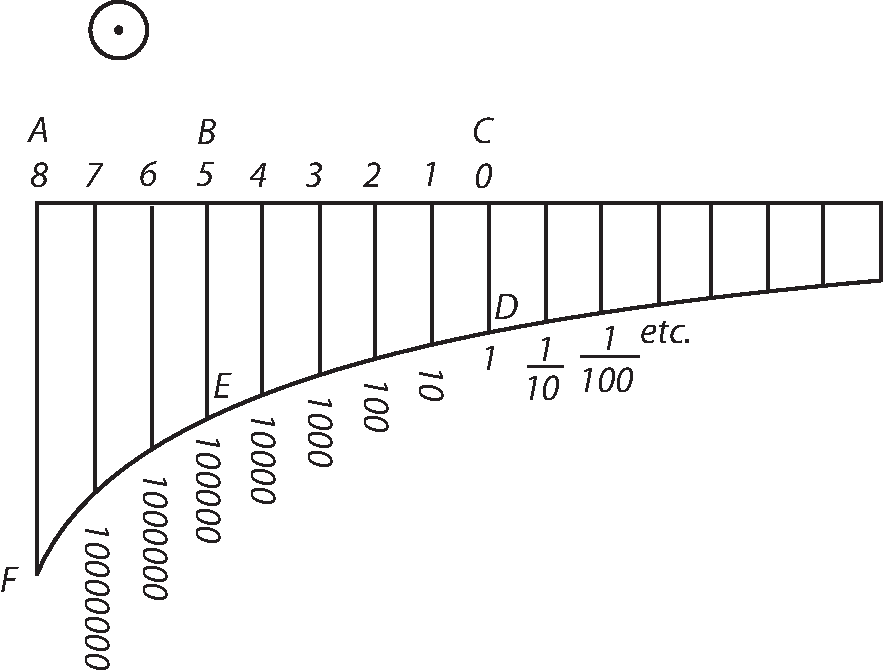
\includegraphics[trim = 0mm -5mm 0mm 0mm, clip, width=0.64\textwidth]{images/lh03705_010v-d1.pdf}
%\pend
%\pstart
% \edtext{}{\lemma{}\killnumber\Afootnote{\textit{Am Rand, unter} [\textit{Fig. 1}]: Videmus corpora ab attritu subito sisti, cum longius itura credi possint, quod fit quia progressio geometrica initio parum, at sub finem valde decrescit, v.g.\textsuperscript{[a]} $\displaystyle 1 \, \cdot \, \frac{1}{10} \, \cdot \, \frac{1}{100} \, \cdot \, \frac{1}{1000} \, \cdot \, \frac{1}{10,000} \, \cdot \, \frac{1}{100,000} \, \cdot $\\% PR: Marginelienapparat.
%\footnotesize \\
%\textsuperscript{[a]} v.g.  \textit{(1)}\ $\displaystyle \frac{7}{10} \, \cdot \, \frac{49}{100} \, \cdot \, \frac{3}{}$ \textit{(2)}\ $\displaystyle 1 \, \cdot \ [...] \ \ \frac{1}{100,000} \, \cdot $ \textit{L}}}
%    \centering
%   \noindent [\textit{Fig. 1}]
%  \pend
%  %\newpage
%\vspace{4mm}
 Geometricae decrescentis per $\displaystyle AF$, $\displaystyle BE$, $\displaystyle CD$, sed crescentis, hinc tamen facile calculari possunt.
Posito enim terminos primum et ultimum pro arbitrio sumtos esse $\displaystyle CD$ et $\displaystyle AF$, data semper \edtext{erit $\displaystyle
CA$. Dato jam}{\lemma{erit $\displaystyle CA$.}\Bfootnote{\textit{(1)}\ Datis autem \textit{(2)}\ Dato jam \textit{L}}}
$\displaystyle BE$, virium
\edtext{detrimento, seu numero, dabitur}{\lemma{detrimento,}\Bfootnote{\textit{(1)}\ dabitur \textit{(2)}\ seu \textit{(a)}\ termino \textit{(b)}\ numero,  \textit{(aa)}\ datur \textit{(bb)}\ dabitur \textit{L}}}
logarithmus ejus ordinarius ex Tabulis: is subtractus a quantitate data constante $\displaystyle AC$, logarithmo scilicet maximo, relinquet $\displaystyle AB$, logarithmum progressionis Geometricae inversae seu decrescentis; ut proinde unica tantum simplici subtractione sit opus.
\pend
\count\Bfootins=1100
\count\Afootins=1100
\newpage
\pstart
\edtext{}{\lemma{}\killnumber\Afootnote{\textit{Am Rand, \"{u}ber} [\textit{Fig. 1}]: Vid. fig. $\rightmoon$\textsuperscript{[a]}. \vspace{2mm}\\% PR: Marginelienapparat.
\footnotesize
\textsuperscript{[a]} fig. $\rightmoon$: [\textit{Fig. 9}] nach unserer Zählung.\vspace{1em}}}
\noindent
\centering 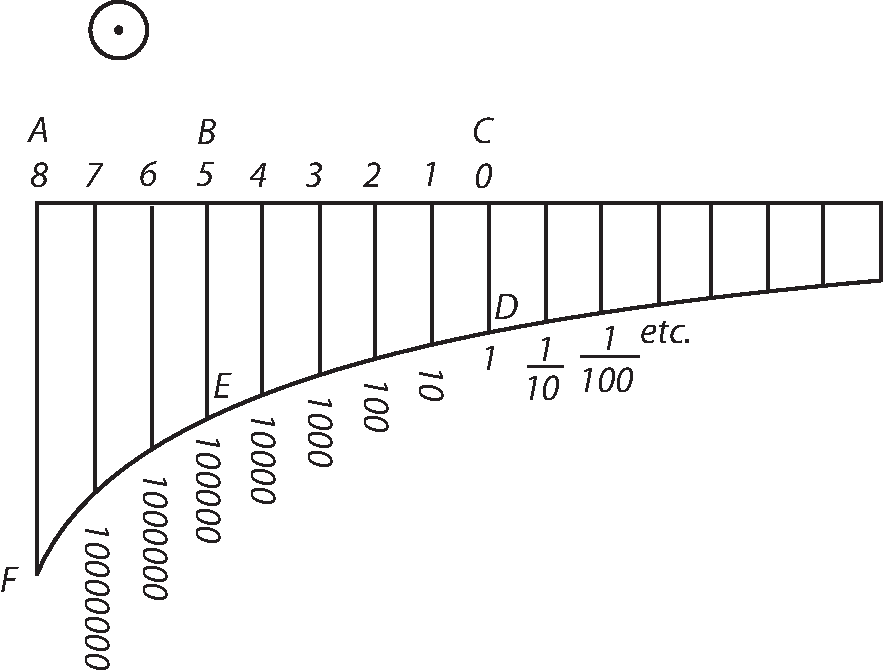
\includegraphics[trim = 0mm -5mm 0mm 0mm, clip, width=0.7\textwidth]{images/lh03705_010v-d1.pdf}
\pend
\pstart
\edtext{}{\lemma{}\killnumber\Afootnote{\textit{Am Rand, unter} [\textit{Fig. 1}]: Videmus corpora ab attritu subito sisti, cum longius itura credi possint, quod fit quia progressio geometrica initio parum, at sub finem valde decrescit, v.g.\textsuperscript{[a]} $\displaystyle 1 \, \cdot \, \frac{1}{10} \, \cdot \, \frac{1}{100} \, \cdot \, \frac{1}{1000} \, \cdot \, \frac{1}{10,000} \, \cdot \, \frac{1}{100,000} \, \cdot $\\% PR: Marginelienapparat.
\footnotesize \\
\textsuperscript{[a]} v.g.  \textit{(1)}\ $\displaystyle \frac{7}{10} \, \cdot \, \frac{49}{100} \, \cdot \, \frac{3}{}$ \textit{(2)}\ $\displaystyle 1 \, \cdot \ [...] \ \ \frac{1}{100,000} \, \cdot $ \textit{L}}}
\centering \noindent [\textit{Fig. 1}]
\pend
\vspace{1.5em}
\pstart
%    \begin{wrapfigure}{l}{0.27\textwidth}
%    \vspace{-4mm}
%    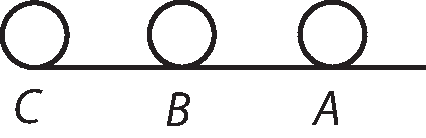
\includegraphics[trim = 0mm -3mm -5mm 0mm, clip, width=0.27\textwidth]{images/lh03705_010v-d2.pdf} %\vspace{0,1mm}\\
%   \centering
%    [\textit{Fig. 2}] % \caption{Bildbeschreibung}
%    \end{wrapfigure}
Porro \setline{1}non detrimenta tantum sed et vires residuae sunt geometricae progressionis, nam habet hoc peculiare sibi geometrica progressio, ut incrementa ejus vel decrementa sint terminis proportionalia.
Porro ad veritatem theorematis per experientiam comprobandam tribus opus est experimentis. %
%\edtext{}{\lemma{}\killnumber\Afootnote{\textit{Am Rand, unter} [\textit{Fig. 2}]: Generaliter\textsuperscript{[a]} Ratio vis in $\displaystyle C$ ad vim in $\displaystyle A$, est multiplicata rationis vis in $\displaystyle B$ ad vim in $\displaystyle A$ in ratione $\displaystyle AC$ ad $\displaystyle AB$. \vspace{2mm}\\%PR: Marginalienapparat.
%\footnotesize
%\textsuperscript{[a]} Generaliter \textit{(1)}\ vis in $\displaystyle A$, ad vim in $\displaystyle C$ \textit{(2)}\ Ratio vis in $\displaystyle C$ ad vim in $\displaystyle A$, \textit{L}\vspace{-4mm}}}
\edtext{Ponatur $\displaystyle AC$ metiri ipsam $\displaystyle AB$}{\lemma{Ponatur}\Bfootnote{\textit{(1)}\ vis in $\displaystyle AC$ esse \textit{(2)}\ $\displaystyle AC$ metiri ipsam $\displaystyle AB$ \textit{L}}},
sit ergo $\displaystyle AB \, \sqcap \, 1$.
$\displaystyle AC$\hfill sit\hfill numerus\hfill integer\hfill $\displaystyle \sqcap \ z$.\hfill
Vis\hfill in\hfill $\displaystyle A$\hfill sit\hfill $\displaystyle a$,\hfill
et\hfill vis\hfill in\hfill $\displaystyle C$,\hfill sit\hfill $\displaystyle c$,\hfill
erit\hfill vis\hfill in\hfill $\displaystyle B$\hfill
\edtext{seu\hfill $\displaystyle b$,}{\lemma{}\Bfootnote{seu $\displaystyle b$, \textit{erg.} \textit{L}}}\hfill
media
\pend
\newpage
\pstart
\noindent
\centering
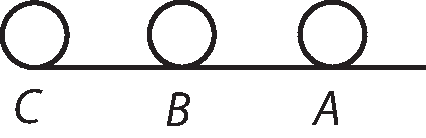
\includegraphics[trim = 0mm -3mm 0mm 0mm, clip, width=0.24\textwidth]{images/lh03705_010v-d2.pdf}\pend
\pstart
\edtext{}{\lemma{}\killnumber\Afootnote{\textit{Am Rand, unter} [\textit{Fig. 2}]: Generaliter\textsuperscript{[a]} Ratio vis in $\displaystyle C$ ad vim in $\displaystyle A$, est multiplicata rationis vis in $\displaystyle B$ ad vim in $\displaystyle A$ in ratione $\displaystyle AC$ ad $\displaystyle AB$. \vspace{2mm}\\%PR: Marginalienapparat.
\footnotesize
\textsuperscript{[a]} Generaliter \textit{(1)}\ vis in $\displaystyle A$, ad vim in $\displaystyle C$ \textit{(2)}\ Ratio vis in $\displaystyle C$ ad vim in $\displaystyle A$, \textit{L}\vspace{-6mm}}}
\noindent \centering
\hspace{-10mm}[\textit{Fig. 2}] 
\pend
\vspace{1.5em}
\pstart \noindent proportionalis \setline{1}inter $\displaystyle a$, et $\displaystyle c$,
secundum numerum $\displaystyle z$, seu
\edtext{$\displaystyle \sqrt{\protect\vphantom{\Large{\scriptstyle\Large h}}}$\!{\protect\textcircled{\Large$\scriptstyle z$}}$\displaystyle ac \sqcap b$. Unde patet}{\lemma{$\displaystyle \sqrt{\protect\vphantom{\Large{\scriptstyle\Large h}}}$\!{\protect\textcircled{\Large$\scriptstyle z$}}$\displaystyle ac \sqcap b$.}\Bfootnote{\textit{(1)}\  sive ut radices evitemus \textit{(2)}\ . Unde patet \textit{L}\hspace{-3mm}}}
hac ratione \edtext{instrumentum fieri posse}{\lemma{instrumentum}\Bfootnote{\textit{(1)}\ reperiri po \textit{(2)}\ fieri posse \textit{L}\hspace{-3mm}}},
cujus ope reperiantur quotcunque mediae proportionales physica constructione.
Si $\displaystyle z \, \sqcap \, 3$ et vis in $\displaystyle A$ ut 1 et vis in $\displaystyle B$ $\displaystyle \, \rule[-4mm]{0mm}{10mm} \frac{1}{4}$
erit vis in $\displaystyle C$ $\displaystyle \sqcap \ \frac{1}{64}$
seu si vis in $\displaystyle A$ $\displaystyle \sqcap \ 1$, vis in $\displaystyle B$ $\displaystyle \sqcap \ b$,
erit vis in $\displaystyle C$ $\displaystyle \sqcap \ b^{z}$. % \pend
[11~r\textsuperscript{o}]
\pend
%\newpage
\count\Bfootins=1200
\count\Afootins=1200
\count\Cfootins=1200
